\documentclass[dvipsnames,border=3pt]{standalone}
\usepackage{tikz}
\usetikzlibrary{arrows}
\usetikzlibrary{shapes}
\usepackage{enumitem}
\usepackage{bm}
\usepackage{mathdots}
\usepackage{amsmath}
\usetikzlibrary{shadings}
\usetikzlibrary{decorations.pathreplacing}
\usepackage{helvet}
\usetikzlibrary{arrows.meta}
\usepackage{graphicx}
\usepackage{pgfplots}
\usepackage{pgfplotstable}
\usepackage{filecontents}
\usetikzlibrary{plotmarks}
\pgfplotsset{compat=newest}

\renewcommand{\familydefault}{\sfdefault}

\definecolor{mylightgray}{cmyk}{0,0,0,0.1}
\usetikzlibrary{arrows,decorations.pathmorphing,backgrounds,fit,positioning,shapes.symbols,chains}

\begin{document}

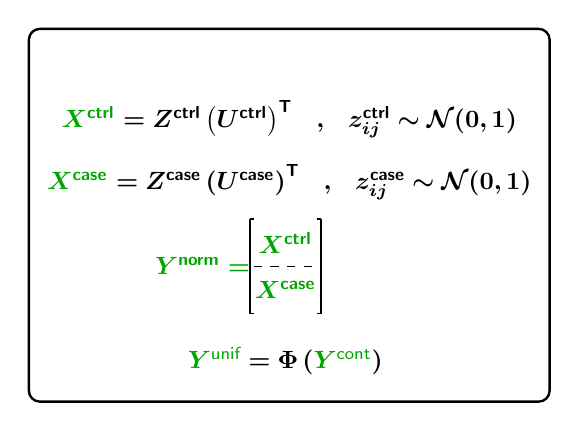
\begin{tikzpicture}
    % trim=left botm right top
    
    %%%%%%%%%%%%%%%%%%%%%%%%%%%%%%%%%%%%%%%%%%%%%%%%%%%%%%%%%%%%%%%%%%%%%%%%%%%%%%%%%%%%%%%%%%%%%%%%%%
    %%%%%%%%%%%%%%%%%%%%%%%%%%%%%%%%%%%%%%%%%%% box 7 %%%%%%%%%%%%%%%%%%%%%%%%%%%%%%%%%%%%%%%%%%%%%%%%
    %%%%%%%%%%%%%%%%%%%%%%%%%%%%%%%%%%%%%%%%%%%%%%%%%%%%%%%%%%%%%%%%%%%%%%%%%%%%%%%%%%%%%%%%%%%%%%%%%%
    
    \node[draw, rounded corners=4, line width=0.3mm, text width=6.38cm, text height=4.5cm] at (9.5,-9.65) {};
    %\node[circle,draw,line width=0.2mm,xscale=1.2,yscale=1.2,fill=GreenYellow] at (7,-7.6) {};
    %\node at (7,-7.6) {\textbf{5}};
    
    %%%%%%%%%%%%%%%%%%%%%%%%%%%%%%%%%%%%%%%%%%%%%%%%%%%%%%%%%%%%%%%%%%%%%%%%%%%%%%%%%%%%%%%%%%%%%%%%%%
    %%%%%%%%%%%%%%%%%%%%%%%%%%%%%%%%%%%%%%%%%%% box 7 %%%%%%%%%%%%%%%%%%%%%%%%%%%%%%%%%%%%%%%%%%%%%%%%
    %%%%%%%%%%%%%%%%%%%%%%%%%%%%%%%%%%%%%%%%%%%%%%%%%%%%%%%%%%%%%%%%%%%%%%%%%%%%%%%%%%%%%%%%%%%%%%%%%%
    
    %%%%%%%%%%%%%%%%%%%%%%%%%%%%%%%%%%%%%%%%%%%%%%%%%%%%%%%%%%%%%%%%%%%%%%%%%%%%%%%%%%%%%%%%%%%%%%%%%%
    %%%%%%%%%%%%%%%%%%%%%%%%%%%%%%%%%%%%%%% correlated data %%%%%%%%%%%%%%%%%%%%%%%%%%%%%%%%%%%%%%%%%%
    %%%%%%%%%%%%%%%%%%%%%%%%%%%%%%%%%%%%%%%%%%%%%%%%%%%%%%%%%%%%%%%%%%%%%%%%%%%%%%%%%%%%%%%%%%%%%%%%%%
    %\node[draw,rounded corners=2,line width=0.2mm,fill=gray!50,text height=0.3cm, text width=2.57cm,shading angle=45] at (9.5,-7.65) {}; % random graph
    %\node at (9.5,-7.65) {\textbf{Correlated Data}};
    
    \node[xscale=0.9,yscale=0.9] at (9.5,-8.43) {\bm{$\textcolor{black!35!green}{X^\textbf{ctrl}}$} \bm{$= Z^\textbf{ctrl} \left(U^\textbf{ctrl}\right)^\textbf{T}$} \hspace{0.1cm} \bm{$,$} \hspace{0.1cm} \bm{$z^\textbf{ctrl}_{ij} \sim \mathcal{N}(0,1)$}};
    
    \node[xscale=0.9,yscale=0.9] at (9.5,-9.23) {\bm{$\textcolor{black!35!green}{X^\textbf{case}}$} \bm{$= Z^\textbf{case} \left(U^\textbf{case}\right)^\textbf{T}$} \hspace{0.1cm} \bm{$,$} \hspace{0.1cm} \bm{$z^\textbf{case}_{ij} \sim \mathcal{N}(0,1)$}};
    
    \node[xscale=0.9,yscale=0.9] at (8.4,-10.3) {\bm{\textcolor{black!35!green}{$Y^\text{norm} =$}}};
    \draw[line width=0.2mm] (9,-10.9) -- (9,-9.7);
    \draw[line width=0.2mm] (9.9,-10.9) -- (9.9,-9.7);
    
    \draw[line width=0.2mm] (9,-10.9) -- (9.05,-10.9);
    \draw[line width=0.2mm] (9,-9.7) -- (9.05,-9.7);
    
    \draw[line width=0.2mm] (9.9,-10.9) -- (9.85,-10.9);
    \draw[line width=0.2mm] (9.9,-9.7) -- (9.85,-9.7);
    
    \draw[line width=0.2mm,dashed] (9.05,-10.3) -- (9.85,-10.3);
    
    \node[xscale=0.9,yscale=0.9] at (9.45,-10) {\bm{\textcolor{black!35!green}{$X^\textbf{ctrl}$}}};
    \node[xscale=0.9,yscale=0.9] at (9.45,-10.6) {\bm{\textcolor{black!35!green}{$X^\textbf{case}$}}};
    
    \node[xscale=0.9,yscale=0.9] at (9.45,-11.5) {\bm{$\textcolor{black!35!green}{Y^\text{unif}}=\Phi \left(\textcolor{black!35!green}{Y^\text{cont}}\right)$}};
    %%%%%%%%%%%%%%%%%%%%%%%%%%%%%%%%%%%%%%%%%%%%%%%%%%%%%%%%%%%%%%%%%%%%%%%%%%%%%%%%%%%%%%%%%%%%%%%%%%
    %%%%%%%%%%%%%%%%%%%%%%%%%%%%%%%%%%%%%%% correlated data %%%%%%%%%%%%%%%%%%%%%%%%%%%%%%%%%%%%%%%%%%
    %%%%%%%%%%%%%%%%%%%%%%%%%%%%%%%%%%%%%%%%%%%%%%%%%%%%%%%%%%%%%%%%%%%%%%%%%%%%%%%%%%%%%%%%%%%%%%%%%%
    
    \end{tikzpicture}
    
\end{document}